% CVPR 2023 Paper Template
% based on the CVPR template provided by Ming-Ming Cheng (https://github.com/MCG-NKU/CVPR_Template)
% modified and extended by Stefan Roth (stefan.roth@NOSPAMtu-darmstadt.de)

\documentclass[10pt,twocolumn,letterpaper]{article}

%%%%%%%%% PAPER TYPE  - PLEASE UPDATE FOR FINAL VERSION
%\usepackage[review]{cvpr}      % To produce the REVIEW version
\usepackage{cvpr}              % To produce the CAMERA-READY version
%\usepackage[pagenumbers]{cvpr} % To force page numbers, e.g. for an arXiv version

% Include other packages here, before hyperref.
\usepackage{graphicx}
\usepackage{amsmath}
\usepackage{amssymb}
\usepackage{booktabs}


% It is strongly recommended to use hyperref, especially for the review version.
% hyperref with option pagebackref eases the reviewers' job.
% Please disable hyperref *only* if you encounter grave issues, e.g. with the
% file validation for the camera-ready version.
%
% If you comment hyperref and then uncomment it, you should delete
% ReviewTempalte.aux before re-running LaTeX.
% (Or just hit 'q' on the first LaTeX run, let it finish, and you
%  should be clear).
\usepackage[pagebackref,breaklinks,colorlinks]{hyperref}


% Support for easy cross-referencing
\usepackage[capitalize]{cleveref}
\crefname{section}{Sec.}{Secs.}
\Crefname{section}{Section}{Sections}
\Crefname{table}{Table}{Tables}
\crefname{table}{Tab.}{Tabs.}


%%%%%%%%% PAPER ID  - PLEASE UPDATE
\def\cvprPaperID{4990} % *** Enter the CVPR Paper ID here
\def\confName{CVPR}
\def\confYear{2026}


\begin{document}

%%%%%%%%% TITLE - PLEASE UPDATE
\title{Plant Disease Detection Using YOLO26 for Real-Time Agricultural Object Detection}
% For a paper whose authors are all at the same institution, omit the following lines up until the closing ``}''.
% Additional authors and addresses can be added with ``\and'', just like the second author.
% To save space, use either the email address or home page, not both
\author{Jonathan Kwong\\
\and
Jared Tan\\
California State Polytechnic University, Pomona\\
{\tt\small https://github.com/Lyrux/plant-disease-detection}
\and
Cole Pedersen\\
}

\maketitle

%%%%%%%%% ABSTRACT
\begin{abstract}
Plant disease detection is a practical computer vision problem for agriculture because early detection can help reduce crop loss and limit disease spread. In this work, we evaluate YOLO26s for strawberry disease detection using a labeled dataset containing seven disease categories. Starting from a baseline configuration of 50 epochs, batch size 16, image size 640, and initial learning rate 0.01, we perform a controlled hyperparameter study by modifying training duration, learning rate, input image size, batch size, and model size. Model performance is evaluated using precision, recall, mAP@50, mAP@50--95, and training and validation loss curves.

Our results show that training duration had the strongest effect on detection performance, with 100 epochs producing the best overall results among the tested epoch settings. Batch size produced moderate improvements, while image size and learning rate had smaller effects on the final validation metrics. The optimized YOLO26s configuration improved precision, recall, mAP@50, and mAP@50--95 compared with the baseline. These results suggest that simple training-parameter changes can improve YOLO26s performance without changing the model architecture.
\end{abstract}

%%%%%%%%% BODY TEXT
\section{Introduction}
\label{sec:intro}

Plant diseases are a major threat to agricultural productivity and crop quality. Infected crops may suffer from reduced yield, lower market value, and, in severe cases, complete crop loss. Traditional disease identification often depends on manual inspection by farmers or agricultural specialists, which can be time-consuming, subjective, and difficult to scale across large farms. This makes automated disease detection a useful computer vision task for agricultural monitoring.

Object detection models are especially useful for this problem because they can both classify the type of disease and localize the affected region in an image. Unlike image classification, which assigns a single label to an entire image, object detection provides bounding boxes around diseased regions. This is useful in real agricultural settings where disease symptoms may appear only on specific leaves, fruits, or small parts of a plant.

In this project, we focus on strawberry disease detection using YOLO26s, a one-stage object detection model. YOLO-based models are well suited for this task because they are designed for efficient detection and can produce bounding box predictions in a single forward pass. Our goal is not to introduce a new model architecture, but to evaluate how different training hyperparameters influence the performance of a YOLO26s detector on plant disease images.

We begin with a baseline YOLO26s configuration using 50 epochs, batch size 16, image size 640, and initial learning rate 0.01. We then modify individual hyperparameters, including the number of epochs, learning rate, image size, and batch size, to measure their effect on training stability and final detection accuracy. By comparing each experiment against the baseline, we identify which hyperparameters have the strongest influence on model performance.

The main contributions of this work are threefold. First, we apply YOLO26s to a strawberry disease detection dataset containing seven disease categories. Second, we perform a controlled hyperparameter study over training duration, learning rate, batch size, and image size. Third, we analyze precision, recall, mAP@50, mAP@50--95, and loss trends to identify which training settings most strongly affect detection performance.

\begin{figure}
    \centering
    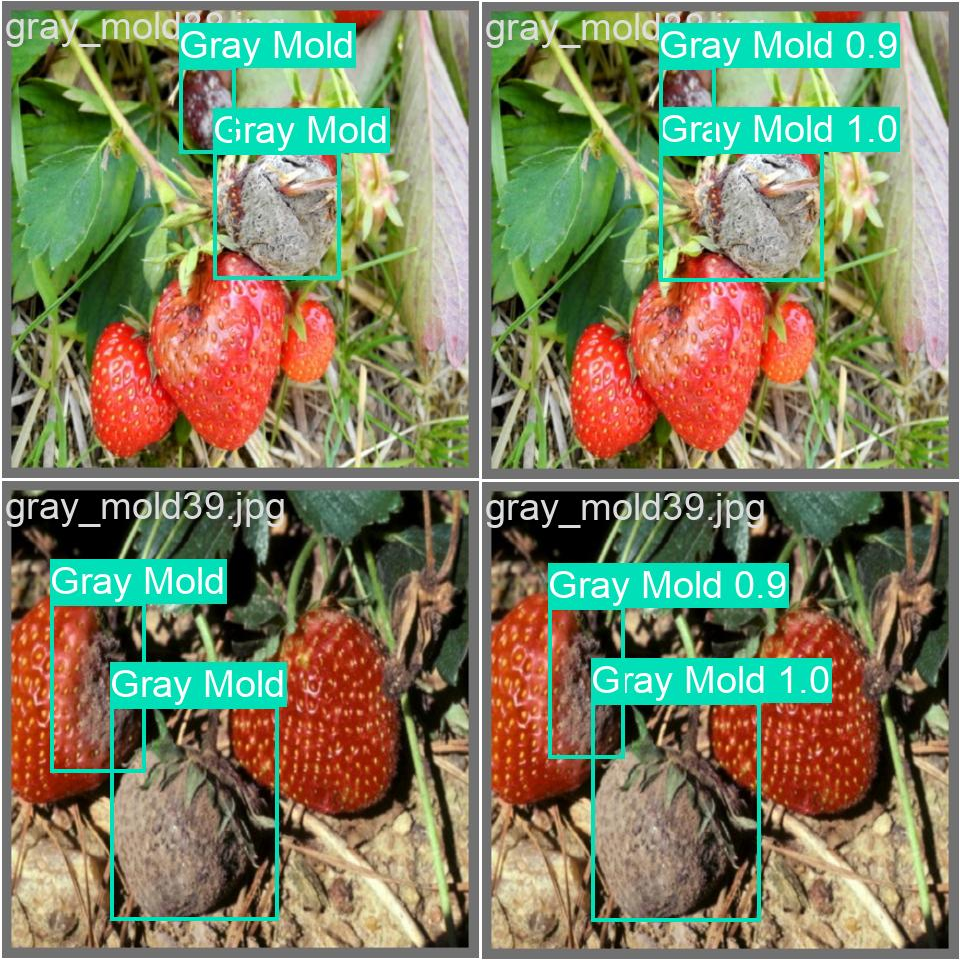
\includegraphics[width=1\linewidth]{images/strawberry detection result.png}
    \caption{Example strawberry disease detection result. The model predicts both the disease class and the bounding box location of the affected plant region.}
    \label{fig:intro_detection_example}
\end{figure}

%------------------------------------------------------------------------
\section{Related Work}
\label{sec:related}

%-------------------------------------------------------------------------
\subsection{Plant Disease Detection}

Plant disease detection has been studied because infections can reduce crop yield and quality. Nazarov et al. report that bacterial, fungal, and viral infections can affect crops at different production stages, with severe cases causing large yield losses~\cite{nazarov2020infectious}. Because symptoms often appear visually through wilting, spotting, mold, rot, discoloration, deformation, or tissue damage, image-based computer vision methods are well suited for disease identification~\cite{nazarov2020infectious}. Traditional diagnosis often depends on manual inspection by farmers or agricultural specialists, but this process can be time-consuming, subjective, and difficult to scale. Recent studies show that computer vision and machine learning can automate plant disease detection by learning disease-related patterns such as lesion texture, fruit damage, mold appearance, and leaf discoloration~\cite{raja2025realtime,upadhyay2025deep}.

%-------------------------------------------------------------------------
\subsection{Object Detection in Agriculture}

Object detection has been widely used in agricultural computer vision tasks such as fruit detection, pest monitoring, weed detection, crop counting, and disease localization. These applications are challenging because agricultural images often contain small targets, occlusion, cluttered backgrounds, changing lighting conditions, and visually similar categories~\cite{upadhyay2025deep}. Page-Fortin et al. note that agricultural targets may also be irregularly shaped and expensive to annotate because expert knowledge is often required~\cite{pagefortin2023class}. Their work is especially relevant because it uses the Strawberry Disease Detection Dataset, which contains 2,500 images across seven strawberry disease categories, and shows that strawberry disease detection is difficult due to limited data, large intra-class variation, and small inter-class differences~\cite{pagefortin2023class}. These challenges motivate the use of object detection instead of image-level classification, since the model must identify both the disease category and the affected region.

%-------------------------------------------------------------------------
\subsection{YOLO-Based Detection}

YOLO models are one-stage object detectors that predict bounding boxes and class probabilities directly from an input image. Compared with two-stage detectors such as Faster R-CNN, one-stage detectors are generally designed for faster inference because they avoid a separate region proposal stage. Upadhyay et al. describe YOLO and SSD as single-stage detectors that estimate bounding boxes and target class probabilities from entire images, making them useful for real-time or near-real-time agricultural applications~\cite{upadhyay2025deep}. Prior agricultural studies have used YOLO-based methods for plant disease and pest detection because they provide a strong balance between speed and detection performance~\cite{upadhyay2025deep}. In this project, YOLO26s is used as the base detector, and performance improvements are studied through hyperparameter tuning rather than architectural modification.

%-------------------------------------------------------------------------
\subsection{Hyperparameter Optimization}

Hyperparameters strongly affect the training behavior and final performance of deep learning models. In object detection, learning rate controls how aggressively model weights are updated, batch size affects the stability of gradient updates, image size determines how much visual detail is preserved, and the number of epochs controls how long the model learns from the dataset. Recent plant disease detection studies commonly evaluate models using precision, recall, F1-score, accuracy, Intersection over Union, and mean Average Precision~\cite{upadhyay2025deep}. Since this project focuses on object detection, the YOLO26s configurations are compared using precision, recall, mAP@50, and mAP@50--95. This allows the study to evaluate how training duration, learning rate, batch size, and image size affect strawberry disease localization and classification performance.

%------------------------------------------------------------------------
\section{Proposed Approach}
\label{sec:approach}

%-------------------------------------------------------------------------
\subsection{Dataset}

The dataset used in this project is the Strawberry Disease Detection Dataset introduced by Afzaal et al.~\cite{afzaal2021strawberry} and made available through Kaggle~\cite{kaggle_strawberry_dataset}. It contains approximately 2,500 labeled disease images across seven disease categories. The disease categories include angular leafspot, anthracnose fruit rot, blossom blight, gray mold, leaf spot, powdery mildew fruit, and powdery mildew leaf. The dataset is relatively small for object detection, which can limit how much information the model is able to learn during training.

Each image contains visual symptoms of strawberry plant disease, and the model is trained to detect these symptoms using object detection annotations. Unlike image classification, where the model predicts only one label for the entire image, object detection requires the model to predict both the disease class and the location of the diseased region. This makes the task more useful for real agricultural applications because it identifies where disease symptoms appear on the plant.

The images are resized during training according to the selected image size hyperparameter. The baseline experiment uses an image size of 640, while additional experiments evaluate smaller and larger image sizes. Image size is important because plant disease symptoms may appear as small spots, discoloration, mold, or localized texture changes. Reducing the image size can remove fine details, while increasing it can preserve more visual information at the cost of greater computational demand.

\begin{figure}
    \centering
    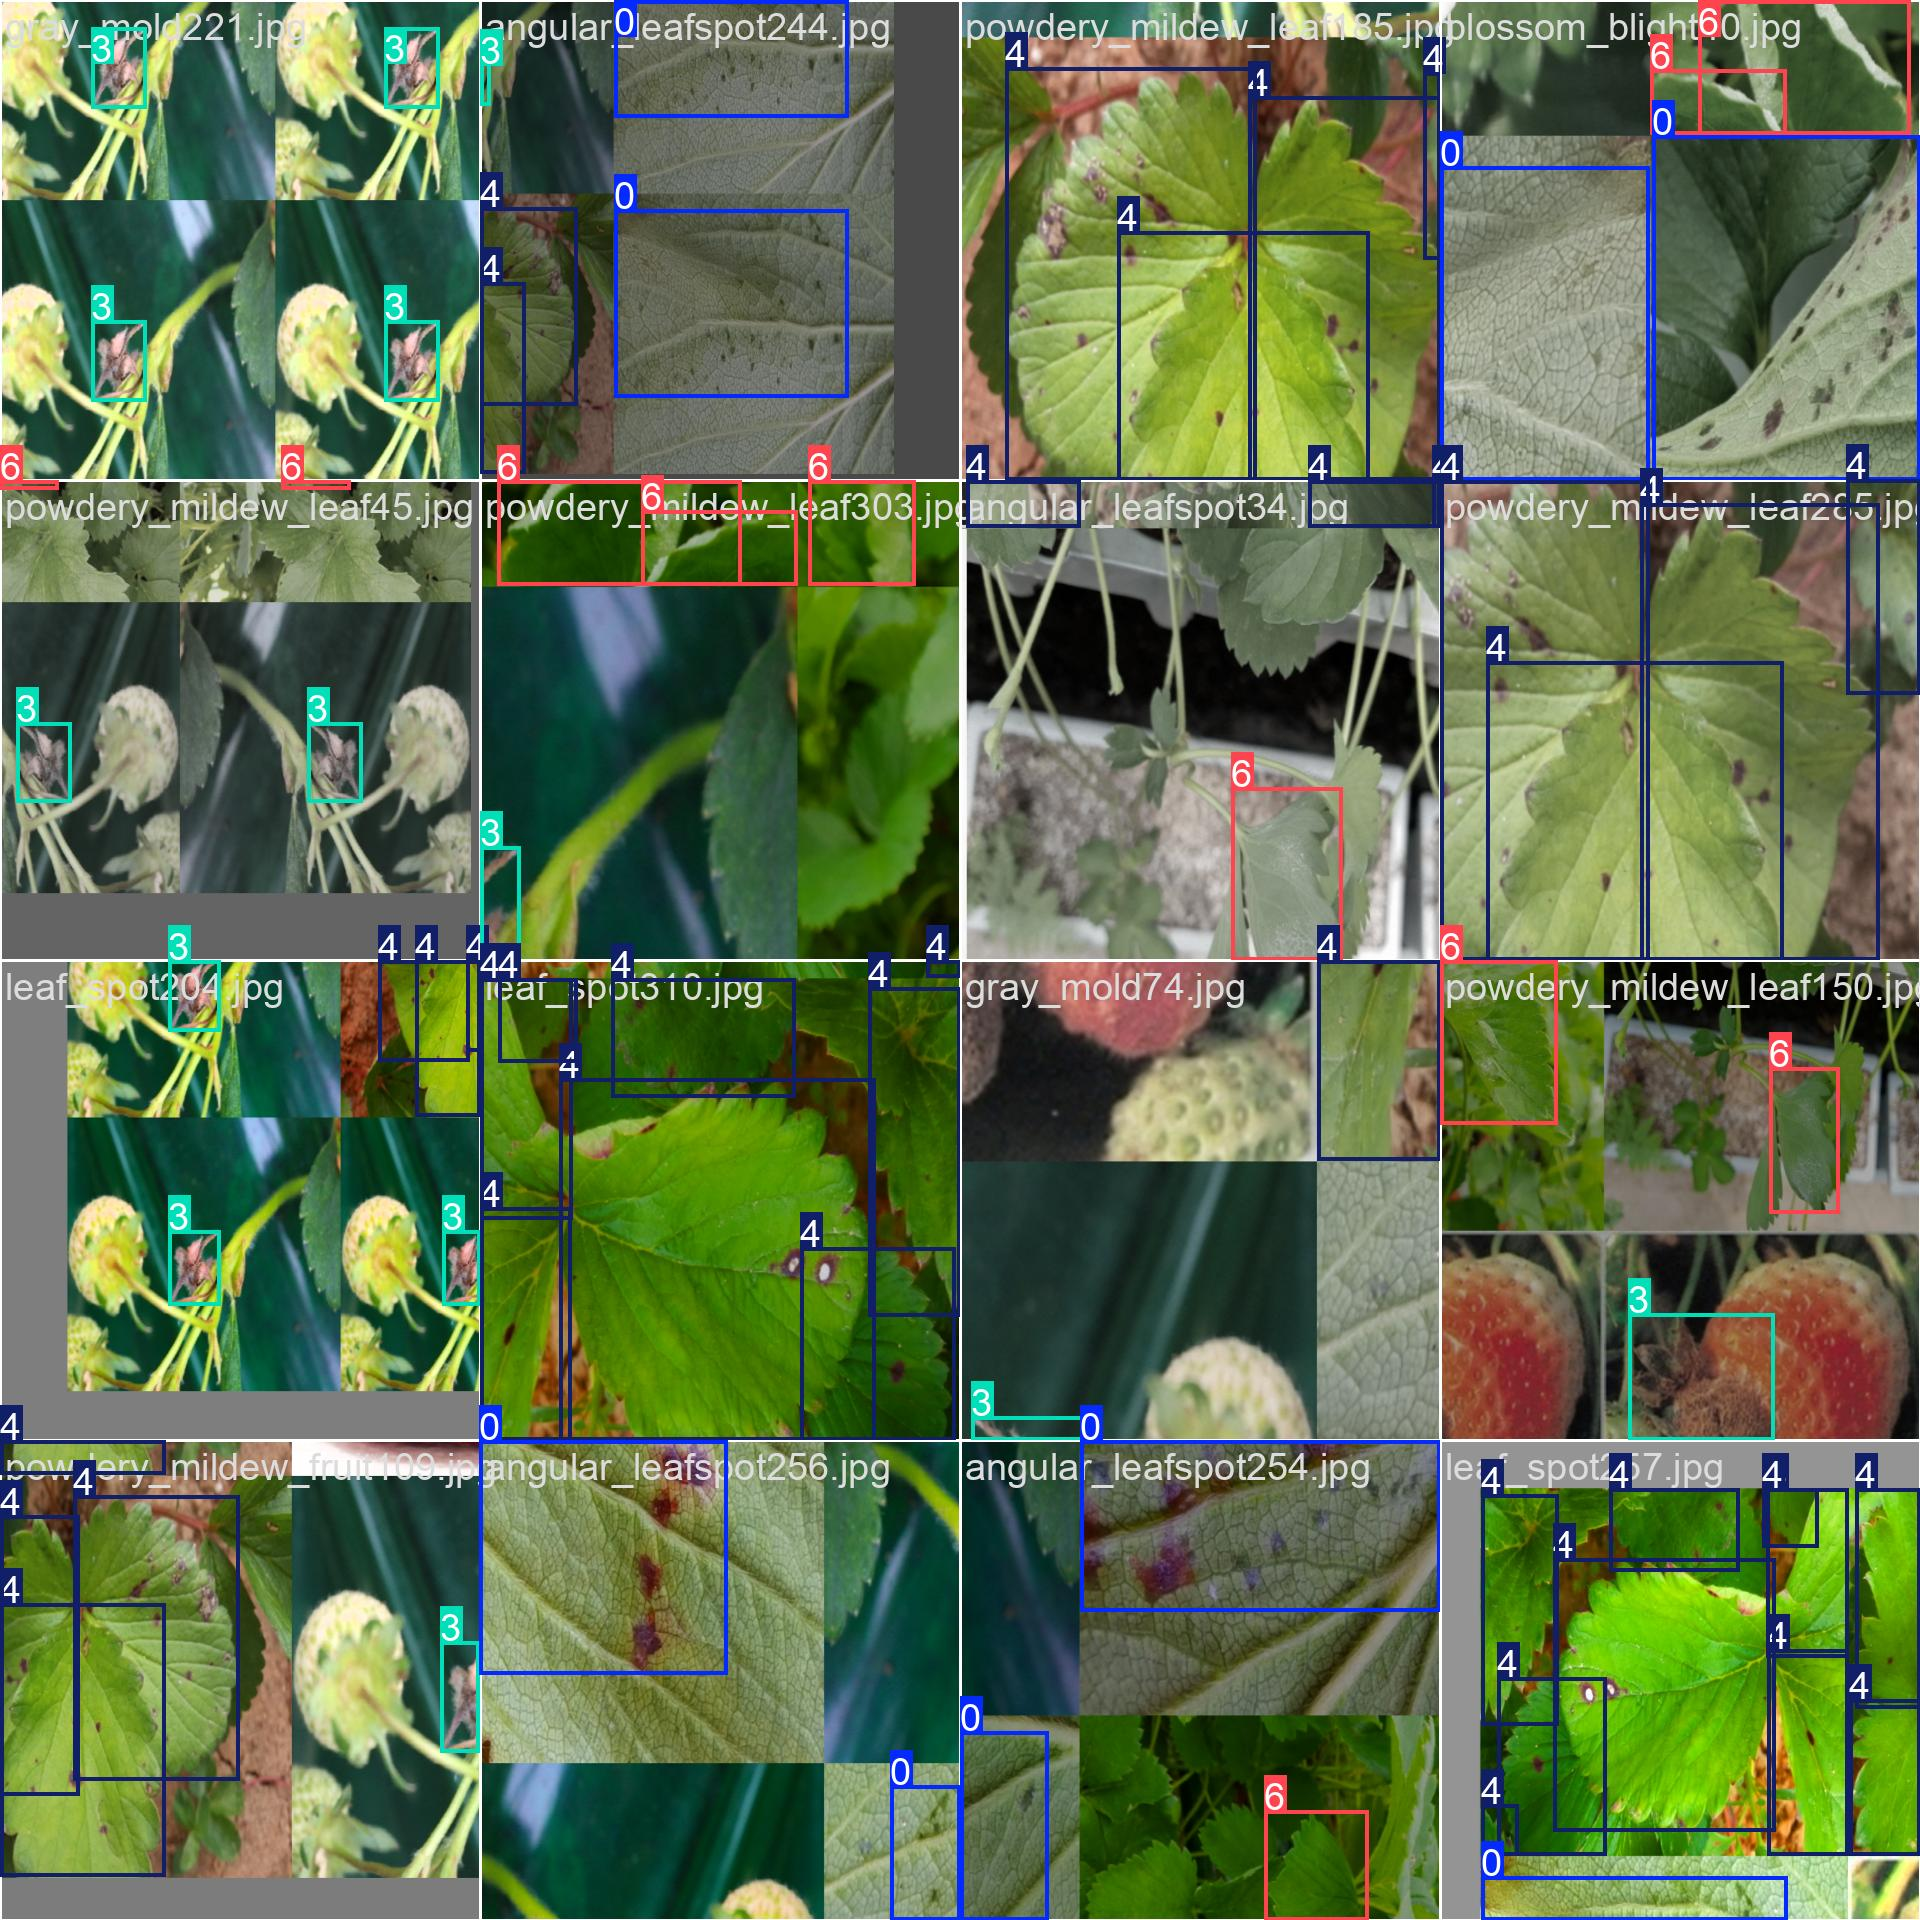
\includegraphics[width=1\linewidth]{images/seven disease category.jpg}
    \caption{Example images from the seven strawberry disease categories used in this study. The classes include angular leafspot, anthracnose fruit rot, blossom blight, gray mold, leaf spot, powdery mildew fruit, and powdery mildew leaf.}
    \label{fig:dataset_class_examples}
\end{figure}

%-------------------------------------------------------------------------
\subsection{Pretrained YOLO26s Baseline Model}

All experiments use YOLO26s as the base model unless otherwise specified. The baseline model serves as the reference point for all experimental comparisons. Each hyperparameter experiment modifies one major training setting while keeping the remaining settings close to the baseline when possible.

During training, the model tracks both training and validation losses, including box loss, classification loss, and distribution focal loss. These losses track localization error, classification error, and bounding box refinement during training. Detection performance is evaluated using precision, recall, mAP@50, and mAP@50--95.

%-------------------------------------------------------------------------
\subsection{YOLO26 Architecture}

The YOLO26 architecture can be broken down into three distinct parts, the head, neck, and backbone. The backbone is responsible for extracting features from the image and feeds multiple layers of the features into the backbone. The backbone then uses these features and aggregates them in order to give the head the data that is required to deduce objects of differing sizes. The head in its base form will use this information to determine three different sizes of objects, small, medium, and large.  This allows the head to accurately detect both individual objects and the many objects that can create a group while keeping in mind data from different layers of the backbone and neck, which allows for greater accuracy.

There are three parameters that control the architecture.  These are the depth multiple, width multiple, and max channels parameter. The depth multiple parameter controls the amount of bottleneck blocks included in the C2PSA module.  Together the width multiple and max channels parameter define the amount of output channels for each block. This controls how much data is output from the C2PSA module allowing for YOLO26 to understand the spacial representation of the image better. For the purposes of this project we will leaving these parameters with their default values.

%-------------------------------------------------------------------------
\subsection{Dataset Preparation}

The original strawberry disease detection dataset contained image files and corresponding JSON annotation files. Before training, the dataset was converted into the YOLO detection format required by the Ultralytics framework. The prepared dataset was organized into separate image and label directories for the training, validation, and testing splits.

Each JSON annotation file contained the image filename, image dimensions, disease class label, and polygon points outlining the diseased region. Since YOLO training requires bounding box annotations, each polygon was converted into a rectangular bounding box by finding the minimum and maximum $x$ and $y$ coordinates of the polygon points. The bounding box was then converted into normalized YOLO format using the class ID, center coordinates, width, and height.

The YOLO label format for each object was written as:
\[
\text{class\_id} \quad x_{\text{center}} \quad y_{\text{center}} \quad w \quad h
\]
where all coordinate values were normalized by the image width and height. Images were copied into the corresponding split directory, and a matching text label file was generated for each image. A \texttt{data.yaml} file was also created to define the dataset path, training, validation, and testing folders, and the seven disease class names.

\begin{table}[!htbp]
  \centering
  \begin{tabular}{@{}cl@{}}
    \toprule
    Class ID & Disease Class \\
    \midrule
    0 & Angular Leafspot \\
    1 & Anthracnose Fruit Rot \\
    2 & Blossom Blight \\
    3 & Gray Mold \\
    4 & Leaf Spot \\
    5 & Powdery Mildew Fruit \\
    6 & Powdery Mildew Leaf \\
    \bottomrule
  \end{tabular}
  \caption{Disease class mapping used for YOLO training.}
  \label{tab:class_mapping}
\end{table}

%-------------------------------------------------------------------------
\subsection{Training Configuration}

The baseline model used \texttt{YOLO26s.pt} with 50 epochs, a batch size of 16, an input image size of 640, and an initial learning rate of 0.01. This baseline configuration was used as the reference point for all hyperparameter comparisons. Unless a parameter was being tested directly, the remaining training settings were kept at their default Ultralytics YOLO values. These included pretrained weights enabled, automatic optimizer selection, mixed precision training enabled, deterministic training enabled, mosaic augmentation set to 1.0, patience set to 100, momentum of 0.937, weight decay of 0.0005, and validation enabled during training.

The hyperparameter study tested changes to the number of epochs, batch size, input image size, initial learning rate, mosaic augmentation, patience, and model size. Model-size experiments compared \texttt{YOLO26n.pt}, \texttt{YOLO26s.pt}, and \texttt{YOLO26m.pt}. After the individual experiments, a final configuration was trained using the best settings from the results.

%-------------------------------------------------------------------------
\subsection{Hyperparameter Tuning Strategy}

The hyperparameter experiments were used to measure which training settings affected YOLO26s performance the most on the strawberry disease dataset. Each run changed one setting from the baseline when possible, including learning rate, batch size, image size, and number of epochs.

The learning rate controls how much the model updates its weights after each optimization step. A learning rate that is too high can make training unstable because the model may update too aggressively and fail to converge smoothly. A learning rate that is too low can make training inefficient because the model learns too slowly and may not reach strong performance within the available number of epochs.

Batch size controls how many images are processed before each model update. A smaller batch size may introduce more variation into the gradient updates, which can make training noisier. A larger batch size may produce smoother training curves, but it can require more GPU memory and may not always improve final performance.

Image size controls the resolution of the images used during training. Larger image sizes preserve more detail, which can help detect small disease symptoms. However, larger images also require more computation. Smaller image sizes reduce training cost but may remove important visual details, especially for diseases that appear as small spots or subtle texture changes.

The number of epochs controls how long the model is trained. Too few epochs may cause underfitting because the model has not had enough time to learn meaningful patterns. More epochs can improve convergence, but excessive training may eventually increase the risk of overfitting.

%-------------------------------------------------------------------------
\subsection{Loss Function}

YOLO26s uses a multi-component object detection loss consisting of bounding box regression, classification loss, and distribution focal loss. The total loss is represented as
\begin{equation}
\mathcal{L}_{total} =
\lambda_{box}\mathcal{L}_{box}
+ \lambda_{cls}\mathcal{L}_{cls}
+ \lambda_{dfl}\mathcal{L}_{dfl},
\end{equation}

where $\mathcal{L}_{box}$ measures localization error, $\mathcal{L}_{cls}$ measures disease classification error, and $\mathcal{L}_{dfl}$ refines bounding box boundary prediction. For the optimized YOLO26s training run, the loss weights were $\lambda_{box}=7.5$, $\lambda_{cls}=0.5$, and $\lambda_{dfl}=1.5$.

%------------------------------------------------------------------------
\section{Results}
\label{sec:results}

%-------------------------------------------------------------------------
\subsection{Experimental Setup}

All experiments were conducted in a Kaggle Notebook environment using an NVIDIA T4 GPU and the Ultralytics YOLO training framework. The strawberry disease detection dataset contains 2,500 labeled images across seven disease categories and is divided into 1,450 training images, 307 validation images, and 743 testing images. The same dataset split was used for every experiment to ensure that performance differences were caused by training configuration changes rather than changes in the data.

\begin{table}[!htbp]
  \centering
  \begin{tabular}{@{}lrr@{}}
    \toprule
    Split & Number of Images & Percentage \\
    \midrule
    Train & 1,450 & 58.0\% \\
    Validation & 307 & 12.3\% \\
    Test & 743 & 29.7\% \\
    \midrule
    Total & 2,500 & 100.0\% \\
    \bottomrule
  \end{tabular}
  \caption{Dataset split for the strawberry disease detection dataset.}
  \label{tab:dataset_split}
\end{table}

Each model was initialized with pretrained weights and trained using the prepared YOLO-format dataset. For each run, performance was evaluated using the metrics generated by the YOLO training process, including training and validation losses, precision, recall, mAP@50, and mAP@50--95. To make the hyperparameter comparisons fair, each experiment changed one setting at a time while keeping the remaining settings fixed to the baseline configuration.

\begin{figure}
    \centering
    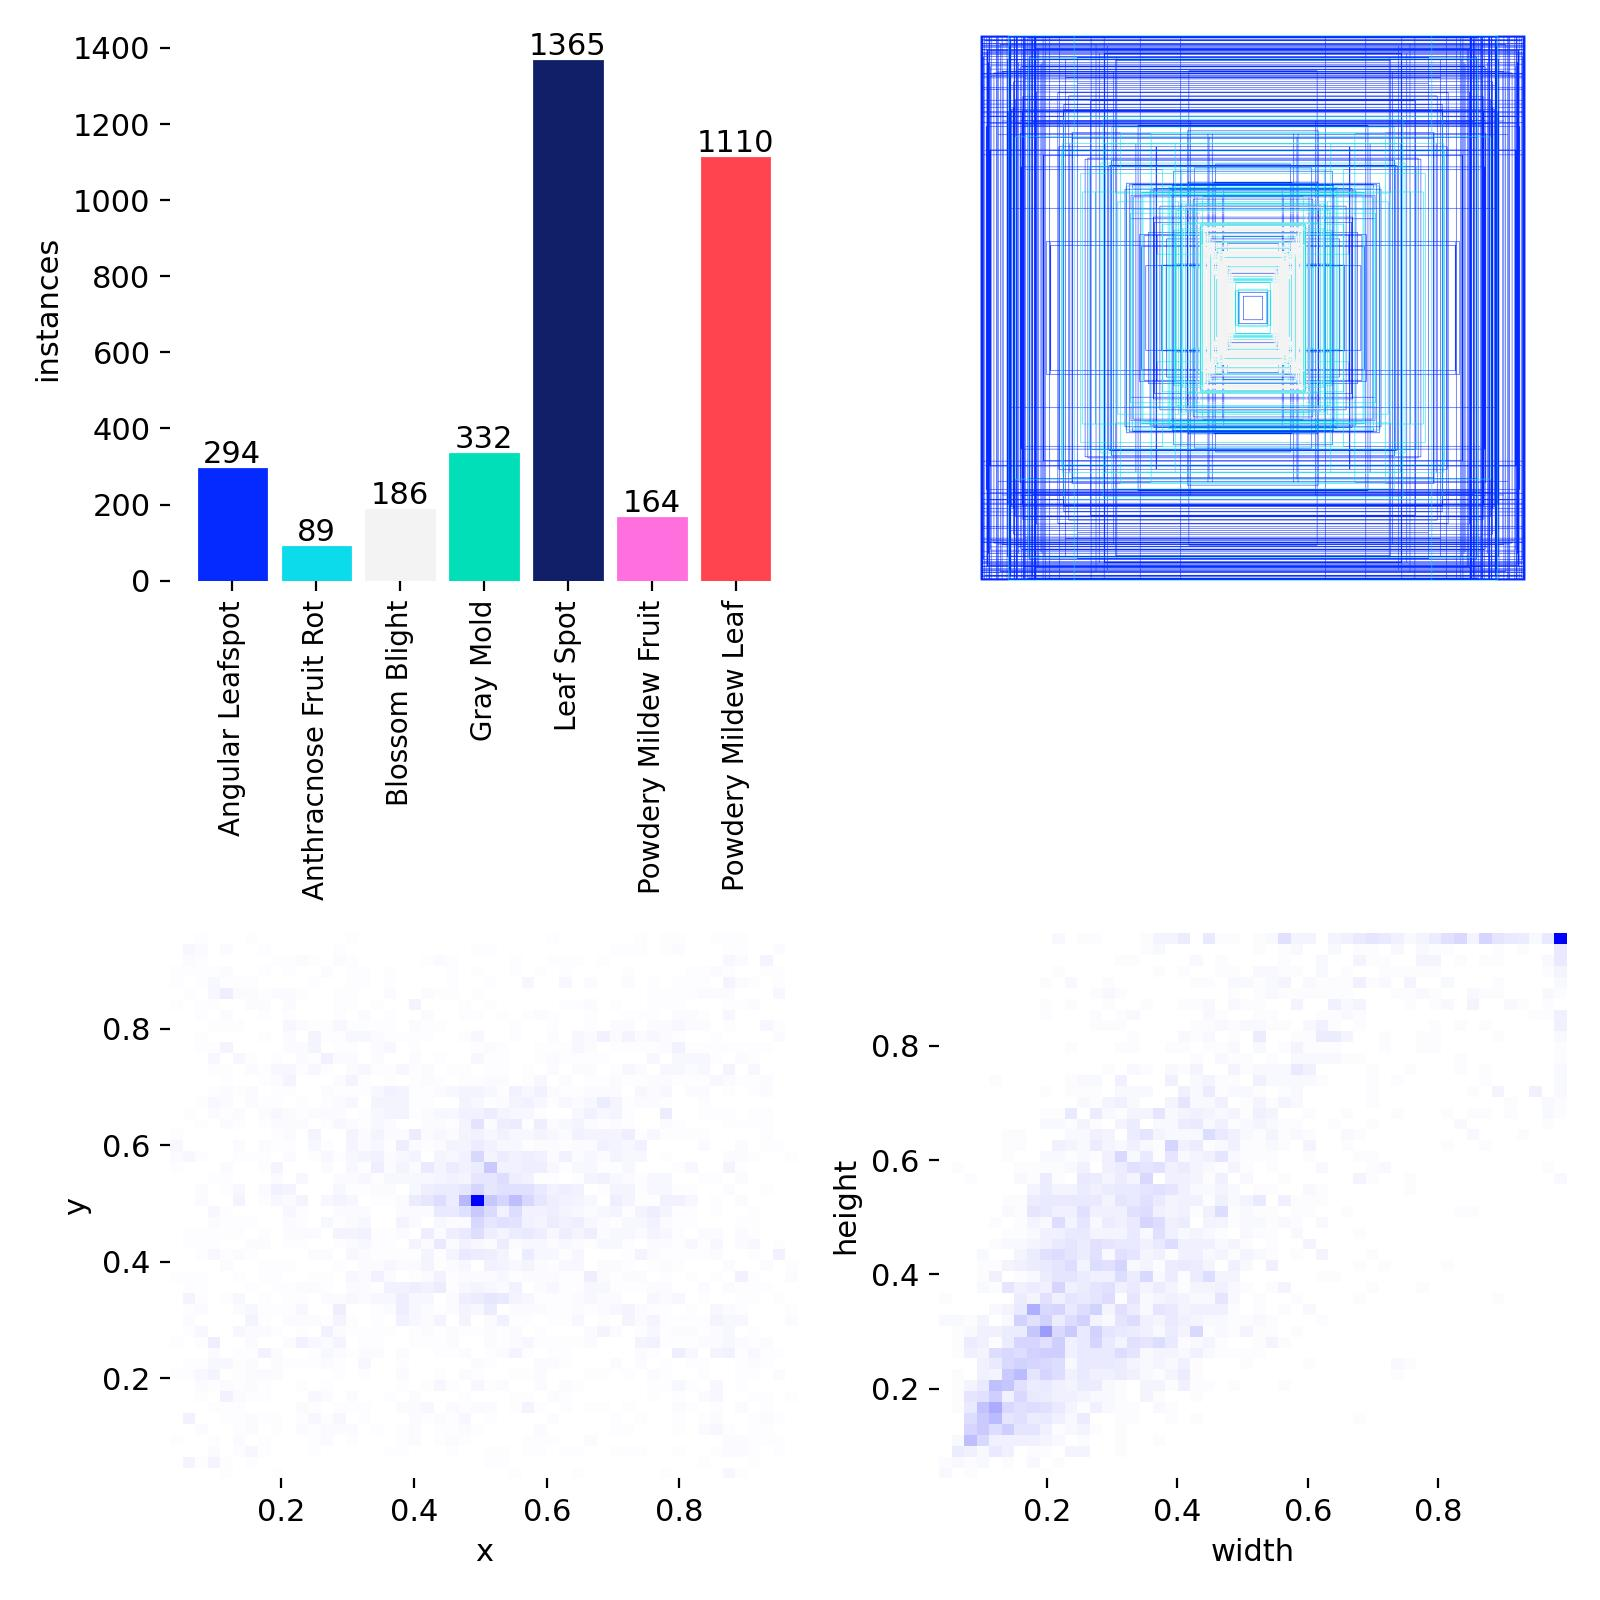
\includegraphics[width=1\linewidth]{images/labels.jpg}
    \caption{Dataset label distribution and bounding-box statistics generated from the YOLO-format strawberry disease dataset.}
    \label{fig:label_distribution}
\end{figure}

\begin{table}[!htbp]
  \centering
  \begin{tabular}{@{}lc@{}}
    \toprule
    Hyperparameter & Baseline Value \\
    \midrule
    Model & YOLO26s.pt \\
    Epochs & 50 \\
    Batch size & 16 \\
    Image size & 640 \\
    Initial learning rate ($lr_0$) & 0.01 \\
    Mosaic & 1.0 \\
    Patience & 100 \\
    \bottomrule
  \end{tabular}
  \caption{Baseline YOLO26s training configuration.}
  \label{tab:baseline_config}
\end{table}

%-------------------------------------------------------------------------
\subsection{Evaluation Metrics}

Detection performance is evaluated using precision, recall, mAP@50, and mAP@50--95. Precision measures the fraction of predicted detections that are correct, while recall measures the fraction of ground-truth objects detected by the model. mAP@50 uses an IoU threshold of 0.50, while mAP@50--95 averages performance across stricter IoU thresholds and provides a stronger measure of localization quality.

%-------------------------------------------------------------------------
\subsection{Baseline Results}

The baseline YOLO26s model was trained using 50 epochs, batch size 16, image size 640, and an initial learning rate of 0.01. This configuration provides the reference point for all later hyperparameter experiments. As shown in Figure~\ref{fig:baseline_training_curves}, the training and validation losses generally decrease over time, while precision, recall, mAP@50, and mAP@50--95 increase throughout training.

This shows that the baseline model learned both disease localization and class prediction successfully from the dataset. However, several metrics continue improving near the end of training, suggesting that the baseline may not be fully converged after 50 epochs. This makes the baseline a useful starting point because it provides stable detection performance while still leaving room for improvement through hyperparameter tuning.

\begin{figure}
    \centering
    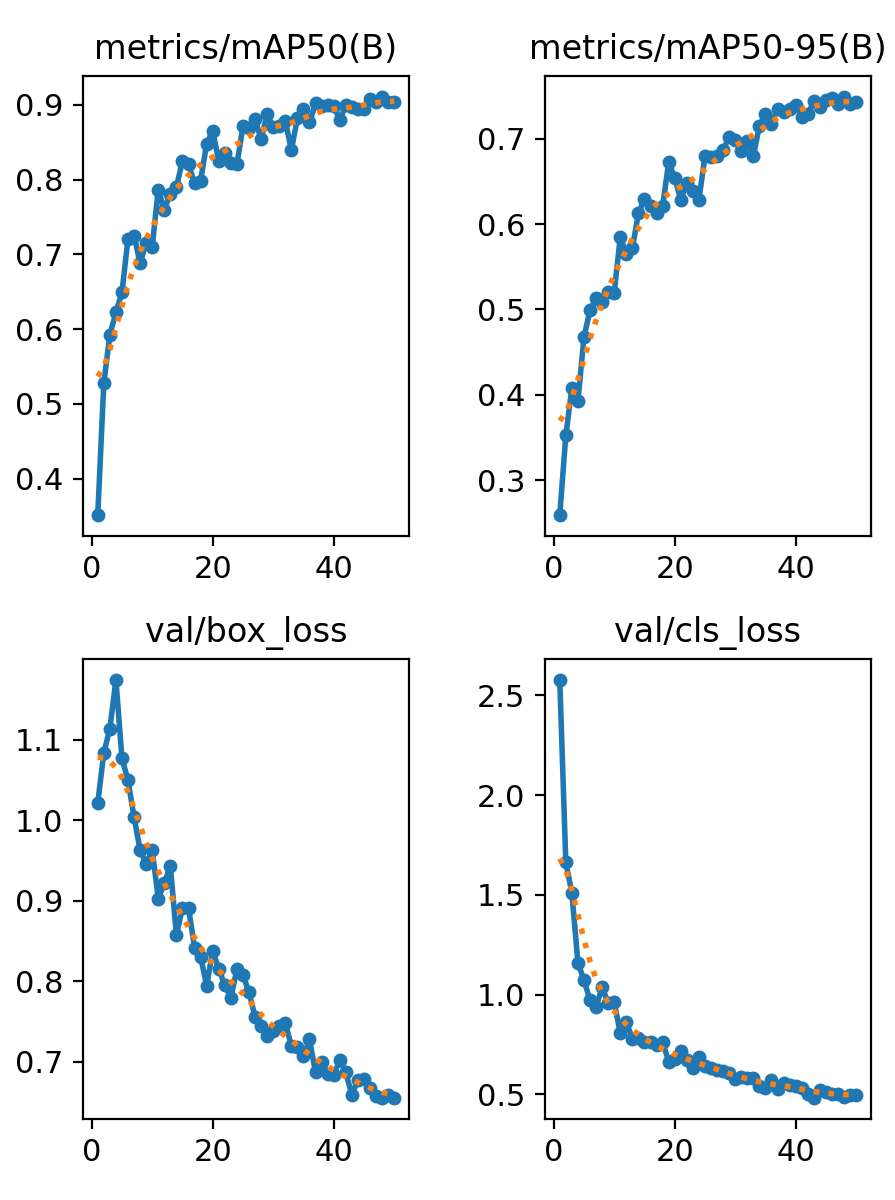
\includegraphics[width=1\linewidth]{images/baseline training curves.png}
    \caption{Baseline YOLO26s training curves using 50 epochs, batch size 16, image size 640, and an initial learning rate of 0.01.}
    \label{fig:baseline_training_curves}
\end{figure}

%-------------------------------------------------------------------------
\subsection{Epoch Comparison}

As shown in Table~\ref{tab:epoch_result}, increasing the number of epochs led to improved detection accuracy for the given model up to 100 epochs. The model achieved its best overall results at 100 epochs, with a precision of 0.908, recall of 0.875, mAP@50 of 0.913, and mAP@50--95 of 0.764. This was likely due to the bounding box approximations becoming more accurate as the model had more time to train and the losses continued to decrease. Decreasing the number of epochs had the opposite effect, as the 10 epoch and 25 epoch runs produced lower detection results because the model most likely did not finish training enough. Increasing the training to 200 epochs did not further improve performance, suggesting that the model had mostly converged by 100 epochs.

\begin{table}[!htbp]
  \centering
  \small
  \begin{tabular}{@{}ccccc@{}}
    \toprule
    Epochs & Precision & Recall & mAP@50 & mAP@50--95 \\
    \midrule
    10  & 0.866 & 0.750 & 0.855 & 0.684 \\
    25  & 0.901 & 0.851 & 0.903 & 0.748 \\
    100 & \textbf{0.908} & \textbf{0.875} & \textbf{0.913} & \textbf{0.764} \\
    200 & 0.908 & 0.874 & 0.902 & 0.755 \\
    \bottomrule
  \end{tabular}
  \caption{Effect of training duration on YOLO26s detection performance.}
  \label{tab:epoch_result}
\end{table}

%-------------------------------------------------------------------------
\subsection{Learning Rate Comparison}

As shown in Table~\ref{tab:lr_result}, changing the initial learning rate did not produce a clear difference in the final detection metrics. The tested learning rates reached nearly the same precision, recall, mAP@50, and mAP@50--95, so lowering or increasing $lr_0$ did not provide a measurable advantage in this experiment. Since the baseline value of $lr_0=0.01$ already produced stable results and did not require additional tuning, it was kept for the optimized configuration.

\begin{table}[!htbp]
  \centering
  \small
  \begin{tabular}{@{}ccccc@{}}
    \toprule
    $lr_0$ & Precision & Recall & mAP@50 & mAP@50--95 \\
    \midrule
    0.0001 & 0.868 & 0.878 & 0.904 & 0.743 \\
    0.001  & 0.868 & 0.878 & 0.904 & 0.743 \\
    1.0    & 0.868 & 0.878 & 0.904 & 0.743 \\
    \bottomrule
  \end{tabular}
  \caption{Effect of initial learning rate on YOLO26s detection performance.}
  \label{tab:lr_result}
\end{table}

%-------------------------------------------------------------------------
\subsection{Image Size Comparison}

As shown in Table~\ref{tab:imgsz_result}, changing the image size had only a small effect on final performance. Increasing the image size to 1024 improved precision and slightly improved mAP@50--95, but recall and mAP@50 were higher at 320. This suggests that the dataset did not require very high input resolution for most detections. However, smaller image sizes can still reduce visual detail and make localization harder for small disease symptoms or visually similar classes.

\begin{table}[!htbp]
  \centering
  \small
  \begin{tabular}{@{}ccccc@{}}
    \toprule
    Image Size & Precision & Recall & mAP@50 & mAP@50--95 \\
    \midrule
    320  & 0.862 & \textbf{0.893} & \textbf{0.911} & 0.740 \\
    1024 & \textbf{0.907} & 0.846 & 0.902 & \textbf{0.744} \\
    \bottomrule
  \end{tabular}
  \caption{Effect of input image size on YOLO26s detection performance.}
  \label{tab:imgsz_result}
\end{table}

%-------------------------------------------------------------------------
\subsection{Batch Size Comparison}

As shown in Table~\ref{tab:batch_result}, changing the batch size produced moderate differences in performance. A batch size of 32 achieved stronger results than a batch size of 8, reaching the highest mAP@50--95 among the batch-size experiments. This suggests that the larger batch size produced more stable updates for this dataset. However, compared with the epoch experiments, batch size had a smaller overall effect on the final optimized configuration.

\begin{table}[!htbp]
  \centering
  \small
  \begin{tabular}{@{}ccccc@{}}
    \toprule
    Batch Size & Precision & Recall & mAP@50 & mAP@50--95 \\
    \midrule
    8  & 0.891 & 0.860 & 0.904 & 0.747 \\
    32 & \textbf{0.930} & \textbf{0.868} & \textbf{0.924} & \textbf{0.771} \\
    \bottomrule
  \end{tabular}
  \caption{Effect of batch size on YOLO26s detection performance.}
  \label{tab:batch_result}
\end{table}

%-------------------------------------------------------------------------
\subsection{Model Size Comparison}

As shown in Table~\ref{tab:model_size_result}, three pretrained YOLO26 model sizes were tested: nano, small, and medium. YOLO26m achieved the best detection performance, while YOLO26n trained the fastest. YOLO26n trained in about 18 minutes, YOLO26s required about 28 minutes, and YOLO26m required about 1 hour and 5 minutes. Although YOLO26m achieved higher accuracy, YOLO26s was selected as the baseline because it provided a better balance between detection performance and training cost.

\begin{table}[!htbp]
  \centering
  \small
  \begin{tabular}{@{}lccccc@{}}
    \toprule
    Model & Precision & Recall & mAP@50 & mAP@50--95 \\
    \midrule
    YOLO26n & 0.888 & 0.844 & 0.903 & 0.739 \\
    YOLO26s & 0.868 & 0.878 & 0.904 & 0.743 \\
    YOLO26m & \textbf{0.902} & \textbf{0.907} & \textbf{0.935} & \textbf{0.776} \\
    \bottomrule
  \end{tabular}
  \caption{Effect of YOLO26 model size on detection performance.}
  \label{tab:model_size_result}
\end{table}

%-------------------------------------------------------------------------
\subsection{Best Configuration}

Based on the results, the optimized configuration used 100 epochs and a batch size of 32 while keeping image size, learning rate, mosaic, and patience unchanged. The number of epochs was increased because the epoch results showed the clearest performance gain. Batch size of 32 was selected because it improved the final metrics without changing the model architecture. Learning rate, image size, mosaic, and patience were kept at their baseline values because they did not provide a consistent improvement. The final optimized configuration is summarized in Table~\ref{tab:config_comparison}.

\begin{table}[!htbp]
  \centering
  \begin{tabular}{@{}lcc@{}}
    \toprule
    Hyperparameter & Baseline Value & Optimized Value \\
    \midrule
    Model & YOLO26s.pt & YOLO26s.pt \\
    Epochs & 50 & 100 \\
    Batch size & 16 & 32 \\
    Image size & 640 & 640 \\
    Initial learning rate ($lr_0$) & 0.01 & 0.01 \\
    Mosaic & 1.0 & 1.0 \\
    Patience & 100 & 100 \\
    \bottomrule
  \end{tabular}
  \caption{Comparison between the baseline and optimized YOLO26s training configurations.}
  \label{tab:config_comparison}
\end{table}

%-------------------------------------------------------------------------
\subsection{Optimized Results}

The optimized configuration used 100 epochs, batch size 32, image size 640, and an initial learning rate of 0.01. Table~\ref{tab:metric_comparison} shows that this configuration produced small improvements across the main detection metrics compared with the baseline. Precision increased from 0.9139 to 0.9310, recall increased from 0.8844 to 0.8973, and mAP@50 increased from 0.9103 to 0.9203. The largest practical gain was in mAP@50--95, which increased from 0.7488 to 0.7580, suggesting improved localization across stricter IoU thresholds.

\begin{table}[!htbp]
  \centering
  \small
  \begin{tabular}{@{}lccc@{}}
    \toprule
    Metric & Baseline & Optimized & Change \\
    \midrule
    Precision & 0.9139 & 0.9310 & +0.0171 \\
    Recall & 0.8844 & 0.8973 & +0.0129 \\
    mAP@50 & 0.9103 & 0.9203 & +0.0100 \\
    mAP@50--95 & 0.7488 & 0.7580 & +0.0092 \\
    \bottomrule
  \end{tabular}
  \caption{Best validation metrics achieved by the baseline and optimized YOLO26s models. Change is reported as absolute difference.}
  \label{tab:metric_comparison}
\end{table}

Table~\ref{tab:loss_comparison} shows that the optimized model reduced most training and localization losses. Training box loss, classification loss, and DFL loss all decreased compared with the baseline. Validation box loss decreased from 0.6556 to 0.6124, and validation DFL loss decreased from 0.0125 to 0.0105. However, validation classification loss increased from 0.4978 to 0.6587, suggesting that the optimized configuration primarily improved localization quality rather than class separation.

\begin{table}[!htbp]
  \centering
  \small
  \begin{tabular}{@{}lccc@{}}
    \toprule
    Loss & Baseline & Optimized & Change \\
    \midrule
    Train box & 0.4530 & 0.3619 & -0.0911 \\
    Train cls & 0.2859 & 0.2012 & -0.0847 \\
    Train DFL & 0.0082 & 0.0064 & -0.0018 \\
    Val box & 0.6556 & 0.6124 & -0.0432 \\
    Val cls & 0.4978 & 0.6587 & +0.1609 \\
    Val DFL & 0.0125 & 0.0105 & -0.0020 \\
    \bottomrule
  \end{tabular}
  \caption{Final training and validation losses for the baseline and optimized YOLO26s models. Change is reported as absolute difference. For losses, negative values indicate improvement.}
  \label{tab:loss_comparison}
\end{table}

%-------------------------------------------------------------------------
\subsection{Limitations}

The main limitation of this project is the dataset size being relatively small, containing approximately 2,500 labeled images. This can limit generalization, especially when disease symptoms vary across lighting conditions, growth stages, and camera viewpoints.

Second, several strawberry disease categories have visually similar symptoms, such as spots, discoloration, or mold-like texture. This makes classification difficult when disease regions are small, partially occluded, or overlapping with natural plant texture. This is consistent with the optimized model results, where localization losses improved but validation classification loss increased.

Third, the improvement from hyperparameter tuning was modest. The optimized configuration improved mAP@50--95 from 0.7488 to 0.7580, but larger gains may require more training data, stronger augmentation, architectural changes, or evaluation on additional plant disease datasets.

%------------------------------------------------------------------------
\section{Conclusion}
\label{sec:conclusion}

This project evaluated YOLO26s for strawberry disease detection using object detection and controlled hyperparameter tuning. Starting from a baseline configuration of 50 epochs, batch size 16, image size 640, and initial learning rate 0.01, we tested changes to training duration, learning rate, batch size, image size, mosaic augmentation, patience, and model size.

The optimized YOLO26s configuration used 100 epochs, batch size 32, image size 640, and initial learning rate 0.01. Compared with the baseline, it improved precision, recall, mAP@50, and mAP@50--95, with the largest practical improvement appearing in mAP@50--95. These results suggest that increasing training duration improved convergence and localization quality, while batch size had a smaller but still useful effect.

The experiments indicate that YOLO26s can detect strawberry disease regions, although the gains from hyperparameter tuning were limited. Future work could improve performance by using a larger dataset, stronger augmentation, additional plant disease datasets, or comparisons with larger YOLO26 variants and other object detection architectures.

For group contributions, Cole conducted architecture research and contributed to the paper. Jared worked on the PowerPoint slides, along with data analysis. Jonathan was responsible for running the training experiments and paper writing. 

%%%%%%%%% REFERENCES
{\small
\bibliographystyle{ieee_fullname}
\bibliography{egbib}
}

\end{document}
